\section{环境和形成路径怎样改变可见性}\label{sec:4-8}

在前述各节的讨论中，原子核的多体波函数、集体形变与跃迁算符通常是在零温自由空间（真空中的裸核多体系统）的微观模型边界下定义的；而实验谱学测量的衰变寿命与分支比，则是在特定的原子与外在介质环境（例如实验室常温下的中性原子、靶基底或晶格介质）中获得的。在第4.6节中，我们讨论了同核异能态的微观阻碍机制——自旋陷阱、Seniority 相消、高 $K$ 空间取向禁戒以及超形变第二极小波函数在变形空间中的位垒穿透压制~\cite{book-jain-nuclear-isomers}；在第4.7节中，探讨了弱衰变算符在有限相空间中的求和定则与有效衰变常数。当把微观核模型导出的核态性质应用于复杂实验与天体物理环境时，需要澄清一种直觉误区：即认为一个同核异能态在实验室中性原子或冷靶环境中拥有长达数小时乃至数年的半衰期，或者拥有更高的微观裂变位垒，便必然能够在高温恒星等离子体中长久存活，或在重离子熔合反应中必然对应更大的产生截面。

原子核在真实物理环境中的有效寿命与在实验谱学中的物理可见性，不是由孤立核哈密顿量单独决定的内禀常数，而是由原子核内禀结构、周围热力学与电磁场环境（辐射场光子密度、原子电离度、电子轨道占有数、晶格介电环境）以及动力学反应形成路径共同塑造的开放动力学过程。同一个核态，在冷真空环境中可能是长寿命异能态，但在高温恒星内部的光子浴中，却可以通过高能中间桥态的热共振激发起发生跨带混合，使有效寿命显著缩短；在原子内转换通道被强电离剥离或受晶格介电禁带压制的环境中，其寿命又可能因电子通道的关闭而延长；而在重离子熔合反应中，高自旋异能组态即使在低温势能面上具有较高的裂变位垒，也并不等同于高温高激发能下复合核的存活几率或最终蒸发剩余核截面会相应增大。

为了建立清晰且定量的物理图像，本节将环境与反应形成对原子核可见性的重塑解构为三个物理子模块：第\ref{sec:4-8-1}小节推演天体等离子体热辐射浴中的开放速率网络、成对可逆电磁跃迁的微观详细平衡边界以及跨簇热化时间尺度；第\ref{sec:4-8-2}小节解构原子核与核外电子通道的微观竞争，系统梳理自发辐射、内转换（IC）、电子俘获核激发（NEEC）、非弹性电子散射（NEIES）与电子跃迁核激发（NEET）等过程，并以 $^{229}\mathrm{Th}$ 光学核钟与 $^{93m}\mathrm{Mo}$ 诱发退激争议为原件实例，确立理论计算与实验证据的边界；第\ref{sec:4-8-3}小节推导重离子完全熔合蒸发反应的三阶段截面分波框架，明确入射势垒穿透、复合核形成与逐级蒸发存活的物理机制与不确定度，并辨析异能态冷态微观位垒与高温反应生成截面之间的逻辑脱耦。图~\ref{fig:4-8-environment-network}给出了这三个子模块的物理机制与特征通道示意图。

\begin{figure}[!htbp]
\centering
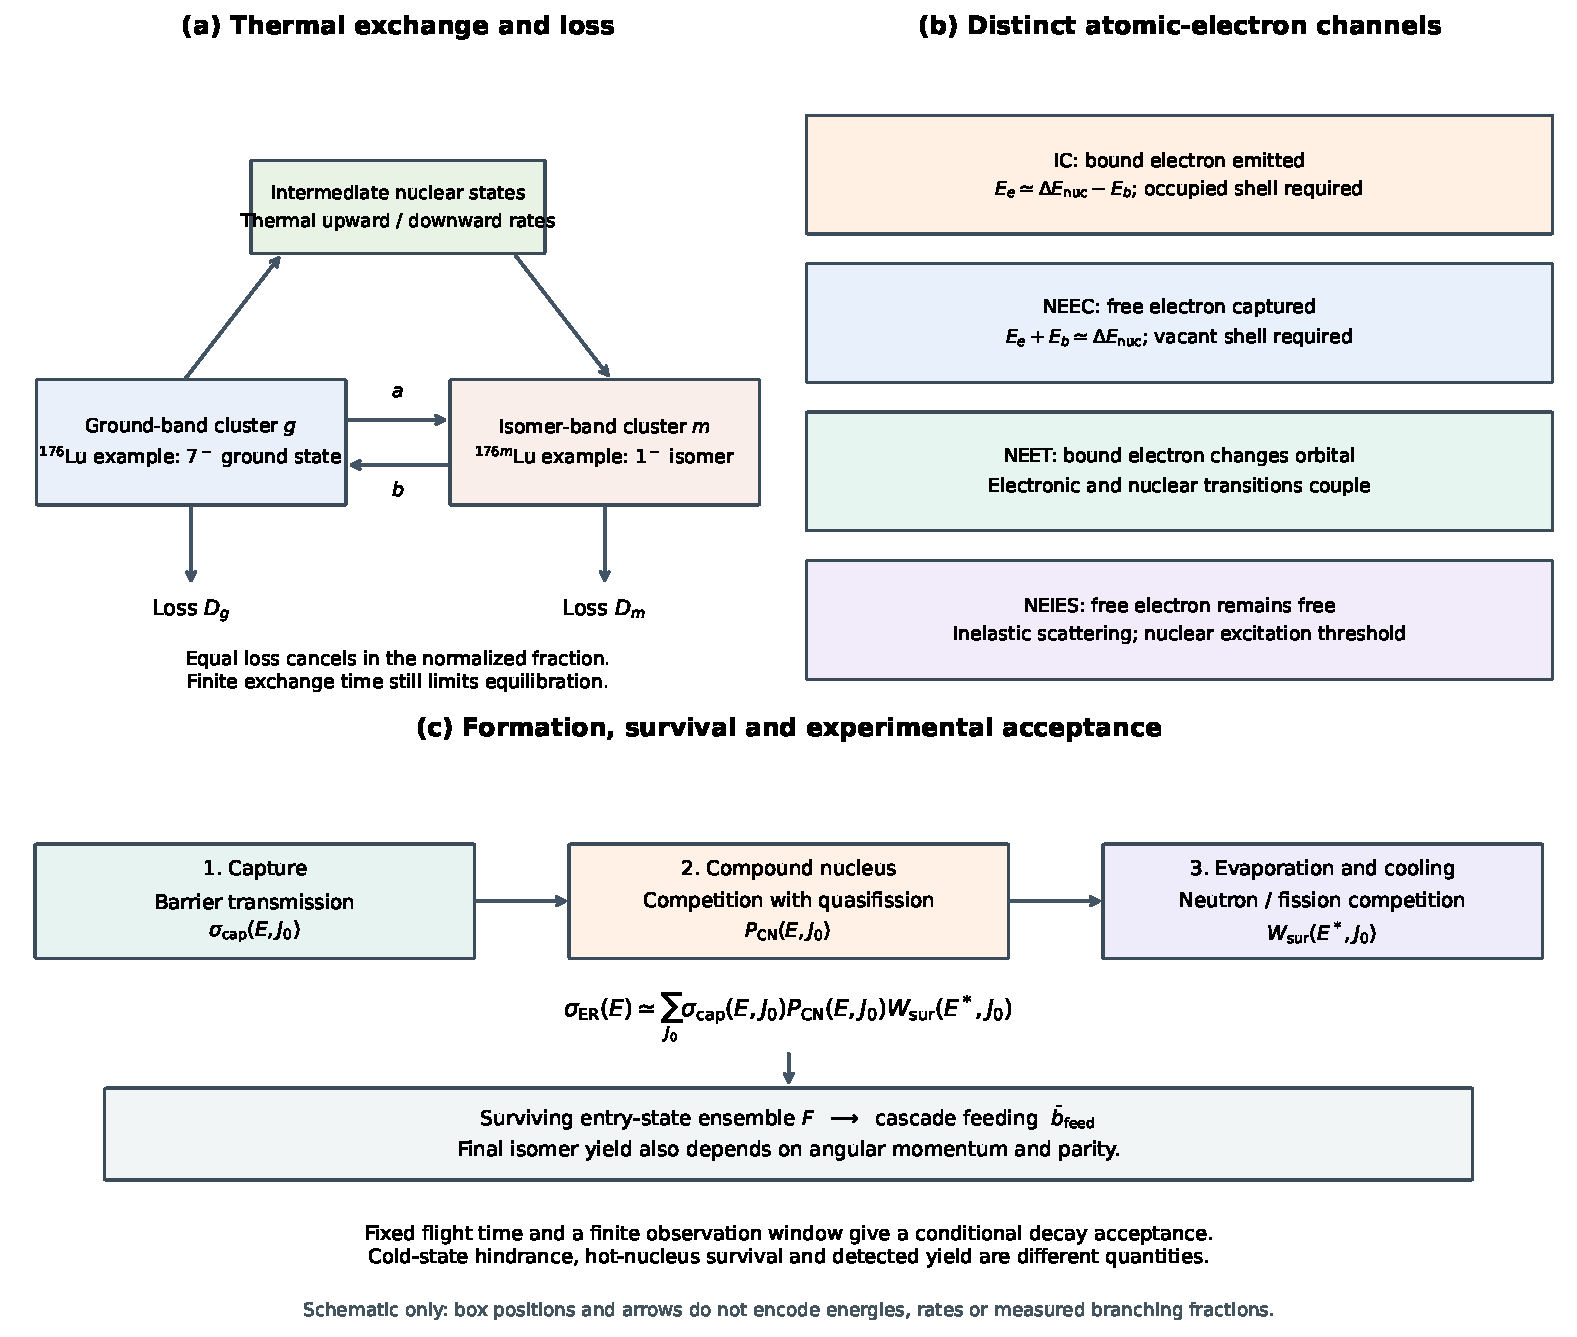
\includegraphics[width=0.98\textwidth]{Img/environment-network-pathways.pdf}
\caption[环境热浴、电子通道与重离子熔合形成对原子核可见性的重塑机制示意图]{环境热浴、电子通道与重离子熔合形成对原子核可见性的重塑机制示意图。(a) 天体热辐射浴中由中间桥态 $|i\rangle$ 介导的基态簇 $g$ 与异能态簇 $m$ 的有效交换网络与本征弛豫尺度；(b) 原子核与核外电子通道的微观竞争机制，包括内转换（IC）、电子俘获核激发（NEEC）、电子跃迁核激发（NEET）与非弹性电子散射（NEIES）；(c) 重离子完全熔合蒸发反应的三阶段分波框架（入射道俘获 $\sigma_{\mathrm{cap}}$、复合核形成 $P_{\mathrm{CN}}$、逐级退激存活 $W_{\mathrm{sur}}$）与进入态系综对异能态的馈入。}\label{fig:4-8-environment-network}
\end{figure}

\subsection{热环境开放网络与有效存活}\label{sec:4-8-1}

在天体物理环境（如渐近巨星分支 AGB 恒星的氦燃烧壳层、$s$-过程核合成温区）中，等离子体温度通常达到 $T_8 \sim 1$--$3$（即 $10^8\ \mathrm{K}$，对应能量标度 $kT \sim 8.6$--$25.9\ \mathrm{keV}$），即 $T_9 \sim 0.1$--$0.3$（$10^9\ \mathrm{K}$）。在这样极端的热力学环境中，原子核浸润在高密度的 Planck 热辐射光子浴以及高温自由电子气体之中。

设某一核素内部存在 $M$ 个离散量子能级（包括基态、低激发态、长寿命异能态以及高激发中间态）。以 $\mathbf{N}(t) = (N_1(t), N_2(t), \dots, N_M(t))^T$ 表示各能级的粒子数密度布居向量（单位为 $\mathrm{cm}^{-3}$）。在恒星核反应网络中，整个原子核能级系统的演化服从一阶非齐次常微分方程组所描述的开放速率网络（Open Rate Network）：
\begin{equation}\label{eq:4-8-network-master}
\frac{d \mathbf{N}(t)}{dt} = \mathbf{A}(T, n_e, \dots) \mathbf{N}(t) + \mathbf{P}(t),
\end{equation}
其中 $\mathbf{P}(t) = (P_1(t), P_2(t), \dots, P_M(t))^T$ 为外部产生流密度向量（例如上一级核反应链或中子俘获对特定能级的直接馈入），而转移矩阵 $\mathbf{A}$ 包含了所有内部能级跃迁与外部破坏漏失：
\begin{equation}\label{eq:4-8-matrix-elements}
A_{ij} = \lambda_{j \to i} \quad (i \ne j), \qquad
A_{ii} = -\sum_{j \ne i} \lambda_{i \to j} - d_i^{\mathrm{sink}}.
\end{equation}
矩阵元具有明确的物理意义与数学约束：
\begin{itemize}
\item \textbf{非对角元的非负性}：对于所有 $i \ne j$，$A_{ij} \ge 0$，表示从能级 $j$ 向能级 $i$ 跃迁的单向速率常数（单位为 $\mathrm{s}^{-1}$）。该跃迁率由光共振吸收、受激/自发辐射以及电子诱发过程共同贡献。
\item \textbf{对角元的外流与漏失}：对角项 $A_{ii} \le 0$ 由流向其他内部能级的总跃迁率以及向核素外部的净漏失率 $d_i^{\mathrm{sink}}$ 构成：
\begin{equation}\label{eq:4-8-sink-def}
d_i^{\mathrm{sink}} \equiv \lambda_{\beta^-}^{(i)} + \lambda_{\beta^+}^{(i)} + \lambda_{\mathrm{EC}}^{(i)} + \lambda_{(n,\gamma)}^{(i)} + \dots \ge 0.
\end{equation}
在此，$d_i^{\mathrm{sink}}$ 包含了从该能级出发导致原子核种类发生改变的所有不可逆弱衰变或核反应通道。
\item \textbf{列和与总核素数密度演化}：对矩阵 $\mathbf{A}$ 的每一列求和可知：
\begin{equation}\label{eq:4-8-column-sum}
\sum_{i=1}^M A_{ij} = A_{jj} + \sum_{i \ne j} A_{ij} = -\left(\sum_{i \ne j} \lambda_{j \to i} + d_j^{\mathrm{sink}}\right) + \sum_{i \ne j} \lambda_{j \to i} = -d_j^{\mathrm{sink}} \le 0.
\end{equation}
对式~\eqref{eq:4-8-network-master}在所有能级上求和，可得总核素数密度 $N_{\mathrm{tot}}(t) = \sum_i N_i(t)$ 的演化方程：
\begin{equation}\label{eq:4-8-total-pop-rate}
\frac{d N_{\mathrm{tot}}}{dt} = -\sum_{i=1}^M d_i^{\mathrm{sink}} N_i(t) + \sum_{i=1}^M P_i(t).
\end{equation}
在系统内部闭合（所有态的外部漏失率均为零，$d_i^{\mathrm{sink}} = 0$）且无外源产生（$\mathbf{P} = 0$）时，转移矩阵每一列和严格为零（$\sum_i A_{ij} = 0$），总核素粒子数密度对任意初值构型均严格守恒。闭合无外源是系统总粒子数对任意初值构型均守恒的充分物理条件；在开放反应网络中，若外部总产生率与总漏失率恰好处于动态平衡（$\sum_i P_i = \sum_i d_i^{\mathrm{sink}} N_i$），特定演化轨迹亦可呈现瞬时变化率为零的平衡态。若要求对于固定的非负常数项 $\mathbf{P}$ 与漏失率 $d_i^{\mathrm{sink}}$，在任意非负初始布居 $\mathbf{N}(0)$ 下均恒有 $d N_{\mathrm{tot}}/dt = 0$，则必须同时具备 $\mathbf{P} = 0$ 且对所有态 $d_i^{\mathrm{sink}} = 0$。
\end{itemize}

在热力学温度为 $T$ 的平衡辐射浴中，能量为 $\Delta = E_u - E_l$ 的光子平均占据数由 Bose-Einstein 统计给出：
\begin{equation}\label{eq:4-8-planck-dist}
n_\gamma(\Delta) = \frac{1}{\exp\left(\frac{\Delta}{kT}\right) - 1}.
\end{equation}
需要指出，$n_\gamma(\Delta)$ 表示每个电磁相空间模的平均光子占据数。在低能极限下（$\Delta \ll kT$），$n_\gamma \approx kT/\Delta$ 可以显著大于 1，不应将其误解为小于等于 1 的概率。

从高能级 $|u\rangle$ 向低能级 $|l\rangle$ 的退激过程由自发辐射与受激辐射共同贡献，其实际总退激跃迁率为：
\begin{equation}\label{eq:4-8-down-trans-rate}
\lambda_{u \to l} = A_{ul} \left[ 1 + n_\gamma(\Delta) \right] = A_{ul} \frac{\exp\left(\frac{\Delta}{kT}\right)}{\exp\left(\frac{\Delta}{kT}\right) - 1}.
\end{equation}
与之对应，从低能级 $|l\rangle$ 吸收环境光子跃迁至高能级 $|u\rangle$ 的光共振吸收跃迁率，由 Einstein 吸收系数与辐射场光子相空间密度导出：
\begin{equation}\label{eq:4-8-up-trans-rate}
\lambda_{l \to u} = \frac{2J_u + 1}{2J_l + 1} A_{ul} n_\gamma(\Delta) = \frac{2J_u + 1}{2J_l + 1} A_{ul} \frac{1}{\exp\left(\frac{\Delta}{kT}\right) - 1}.
\end{equation}
将式~\eqref{eq:4-8-up-trans-rate}与式~\eqref{eq:4-8-down-trans-rate}直接相除，即可得到成对电磁跃迁率的比例关系：
\begin{equation}\label{eq:4-8-detailed-balance-em}
\frac{\lambda_{l \to u}}{\lambda_{u \to l}} = \frac{2J_u + 1}{2J_l + 1} \exp\left(-\frac{\Delta}{kT}\right) = \frac{2J_u + 1}{2J_l + 1} \exp\left(-\frac{E_u - E_l}{kT}\right).
\end{equation}

式~\eqref{eq:4-8-detailed-balance-em}表述的是在 Planck 热辐射浴中，成对可逆电磁跃迁所严格遵循的微观详细平衡。然而，这一局域关系并不能等同于整个开放原子核网络必然服从宏观热平衡或全局 Boltzmann 统计分布：
\begin{equation}\label{eq:4-8-boltzmann-naive}
\frac{N_m}{N_g} \stackrel{?}{=} \frac{2J_m + 1}{2J_g + 1} \exp\left(-\frac{E_m - E_g}{kT}\right).
\end{equation}
全局平衡的破坏主要源于以下机制：
\begin{enumerate}
\item \textbf{非对称弱衰变漏失}：基态与异能态的核自旋、宇称与内部波函数构型往往存在剧烈差异，导致二者的 $\beta$ 衰变或电子俘获速率相差数个至十数个数量级（即 $d_g^{\mathrm{sink}} \ne d_m^{\mathrm{sink}}$）。弱衰变是向体系外部连续排泄布居的单向不可逆流动，破坏了全网络的封闭性。
\item \textbf{外源非平衡馈入}：上一级核反应链（例如中子俘获反应 $(n,\gamma)$）对各能级的馈入截面并不服从温度 $T$ 的热力学配分，而是由中子共振能级波函数决定（即 $P_g(t) / P_m(t)$ 不等于热平衡权重）。
\item \textbf{跨带耦合速率与有限热化时间}：带内能级由于较强的电磁跃迁，在光子浴驱动下可较快建立局域热平衡；但低自旋基态与高自旋（或大 $K$ 差）异能态之间的直接电磁跃迁受到强烈禁戒。两态之间的热交换必须依赖能量更高的非禁戒中间桥态进行多步跃迁，其有效交换速率有限。如果恒星环境温度演化时间尺度或核素破坏时间尺度短于跨带热化时间尺度，系统将始终处于动力学偏离平衡状态。
\item \textbf{弱相互作用透明性条件}：在典型 $s$-过程恒星演化壳层中，中微子平均自由程远大于恒星核尺寸，中微子流自由逸出，逆中微子吸收过程可以忽略；而在超新星坍缩等中微子不透明致密环境中，中微子相空间分布将直接介入反应网络，需要额外计入弱相互作用的非平衡输运。
\end{enumerate}

在物理上，我们可以将属于基态转动带的所有快速热平衡能级归并为基态簇（Ground Cluster，总布居记为 $N_g$），将属于异能态转动带的所有能级归并为异能态簇（Isomer Cluster，总布居记为 $N_m$）。带内能级由于纳秒或亚纳秒级的电磁退激，在高温光子浴提供充足向上激发的条件下可迅速建立局域热配分分布。定义有效跨簇交换率 $a \equiv \lambda_{g \to m}^{\mathrm{eff}}$ 与 $b \equiv \lambda_{m \to g}^{\mathrm{eff}}$，以及各簇的热加权有效破坏漏失率 $D_g$ 与 $D_m$（主要由各态的 $\beta$ 衰变贡献），双簇开网络方程可写为：
\begin{equation}\label{eq:4-8-two-cluster-master}
\frac{d}{dt}\begin{pmatrix} N_g(t) \\ N_m(t) \end{pmatrix} =
\begin{pmatrix} -(a + D_g) & b \\ a & -(b + D_m) \end{pmatrix}
\begin{pmatrix} N_g(t) \\ N_m(t) \end{pmatrix} +
\begin{pmatrix} P_g(t) \\ P_m(t) \end{pmatrix}.
\end{equation}

在恒定环境条件且无外部连续产生（$\mathbf{P} = 0$）的条件下，式~\eqref{eq:4-8-two-cluster-master}的演化由双态有效转移矩阵的特征值决定。设解的形式包含衰减因子 $e^{-r t}$，特征方程给出两个衰减特征值 $r_\pm$：
\begin{equation}\label{eq:4-8-cluster-eigenvalues}
r_\pm = \frac{1}{2}\left\{ (a + b + D_g + D_m) \pm \sqrt{(a + D_g - b - D_m)^2 + 4ab} \right\}.
\end{equation}
对式~\eqref{eq:4-8-cluster-eigenvalues}进行深入的物理极限与时间尺度分析：
\begin{enumerate}
\item \textbf{等漏失极限下的热化时间尺度}：当两簇的外部漏失率相等（$D_g = D_m = D$）时，根号内部化简为 $\sqrt{(a-b)^2 + 4ab} = a+b$。此时两个特征值为：
\begin{equation}\label{eq:4-8-lossless-limits}
r_- = D, \qquad r_+ = a + b + D.
\end{equation}
特征值之差严格为 $r_+ - r_- = a + b$。此时系统的总数按共同速率 $D$ 衰减，若考察归一化相对布居份额 $f \equiv N_m / (N_g + N_m)$，直接由式~\eqref{eq:4-8-two-cluster-master}求导可知 $D$ 项在归一化方程中严格相消：
\begin{equation}\label{eq:4-8-normalized-fraction-ode}
\frac{df}{dt} = a - (a + b)f - (D_m - D_g)f(1 - f) + \frac{P_m - f(P_g + P_m)}{N_{\mathrm{tot}}}.
\end{equation}
当 $D_g = D_m$ 且 $\mathbf{P} = 0$ 时，非线性选择项与外源项同时为零，归一化份额 $f(t)$ 严格按速率 $a + b$ 指数弛豫至平衡比 $a/(a+b)$。因此，在等漏失条件下，特征热化平均时间尺度表示为：
\begin{equation}\label{eq:4-8-therm-timescale}
\tau_{\mathrm{therm}} = \frac{1}{a + b} = \frac{1}{\lambda_{g \to m}^{\mathrm{eff}} + \lambda_{m \to g}^{\mathrm{eff}}},
\end{equation}
其对应的半平衡时间为 $t_{1/2}^{\mathrm{therm}} = \tau_{\mathrm{therm}} \ln 2 = \frac{\ln 2}{a + b}$。
严格闭合无损失的体系（$D_g = D_m = 0$）是该极限中 $r_- = 0$ 的充分特例，但并非唯一的物理适用条件。在常系数矩阵（恒温）且无外源（$\mathbf{P} = 0$）条件下，即便两簇存在非对称漏失（$D_g \ne D_m$），该线性自治系统仍可通过特征值与特征向量解析展开为 $\mathbf{N}(t) = \exp(\mathbf{A}t)\mathbf{N}_0$；然而此时系统的慢衰减特征模将偏离简单的 $a+b$。若环境温度随时间演化导致转移矩阵时变 $\mathbf{A}(t)$，或存在随时间变化的外源馈入流 $\mathbf{P}(t)$，系统将成为非自治微分方程组，瞬时单一有效寿命通常不足以描述整体布居动力学，应求解完整网络（数值求解或适当的解析卷积）。
\item \textbf{快速热化弱漏失极限下的有效衰变率}：当温度升高使得通过桥态的热激发交换率远大于两簇的弱衰变差异（即 $a + b \gg |D_g - D_m|$）时，较小特征值 $r_-$ 可以通过关于漏失差的微扰展开近似为：
\begin{equation}\label{eq:4-8-effective-decay-approx}
r_- \simeq D_{\mathrm{eff}} = \frac{b D_g + a D_m}{a + b}.
\end{equation}
在此极限下，成对电磁跃迁建立微观详细平衡，跨簇有效交换率之比趋向于簇配分函数加权比：
\begin{equation}\label{eq:4-8-partition-ratio}
\frac{a}{b} = \frac{\lambda_{g \to m}^{\mathrm{eff}}}{\lambda_{m \to g}^{\mathrm{eff}}} \simeq \frac{Z_m(T)}{Z_g(T)} \exp\left(-\frac{E_m - E_g}{kT}\right),
\end{equation}
其中 $Z_g(T) = \sum_{j \in g} (2J_j + 1) e^{-(E_j - E_g)/kT}$ 与 $Z_m(T) = \sum_{k \in m} (2J_k + 1) e^{-(E_k - E_m)/kT}$ 分别为基态簇与异能态簇的内部配分函数。将式~\eqref{eq:4-8-partition-ratio}代入式~\eqref{eq:4-8-effective-decay-approx}，全系统的宏观有效衰变破坏率表现为热加权平均形式：
\begin{equation}\label{eq:4-8-therm-decay-average}
D_{\mathrm{eff}}(T) \simeq \frac{Z_g(T) D_g + Z_m(T) e^{-(E_m - E_g)/kT} D_m}{Z_g(T) + Z_m(T) e^{-(E_m - E_g)/kT}}.
\end{equation}
但必须指出，微扰条件 $a + b \gg |D_g - D_m|$ 仅保证了长时间渐近衰减率可展开为热加权形式 $D_{\mathrm{eff}}$；在有限的恒星脉冲温区或实验观测时间窗内，系统是否真正达到这一热平衡布居，还强烈依赖于初始注入条件在快模 $r_+$ 与慢模 $r_-$ 上的投影分布，以及跨带特征交换时间 $\tau_{\mathrm{therm}} = 1/(a+b)$ 相对天体流体冷却时间或反应时间的大小。如果交换时间长于环境演化时间，原子核在尚未建立热平衡之前就可能已经发生严重的不平衡衰变漏失。
\end{enumerate}

天体核合成中一个代表性的理论模型实例是 $s$-过程核素 $^{176}\mathrm{Lu}$ 的跨带热化（Gintautas 等人 2009~\cite{gintautas-2009-176lu-thermal-equilibration}，Gosselin 等人 2010~\cite{gosselin-2010-plasma-isomers-176lu-180ta}）。在此需要强调，Gintautas 等人（2009）是基于 ENSDF 评估能级参数开展的跃迁速率与 $K$ 混合理论模型计算，而非给出新的直接实验测定。根据该文原件核定（PDF 第2页第II节开头），$^{176}\mathrm{Lu}$ 的基态为 $J^\pi = 7^-$（$K^\pi = 7^-$），具有长达 $T_{1/2} = 3.76 \times 10^{10}\ \mathrm{yr}$（平均寿命 $\tau \approx 5.42 \times 10^{10}\ \mathrm{yr}$）的弱衰变半衰期；而其激发能为 $122.9\ \mathrm{keV}$ 的同核异能态 $^{176m}\mathrm{Lu}$ 自旋宇称为 $J^\pi = 1^-$（$K^\pi = 0^-$），主要通过 $\beta^-$ 衰变到 $^{176}\mathrm{Hf}$（根据 NNDC/ENSDF 评估数据集~\cite{nndc-176lu-beta-2006-snapshot}，优势分支馈入 $^{176}\mathrm{Hf}$ 的 $0^+$ 基态与 $88.4\ \mathrm{keV}$ $2^+$ 能级，分支比分别约为 $39(2)\%$ 与 $61(2)\%$；由 $1^-$ 母态出发因宇称改变，属于一阶禁戒非唯一型跃迁，而非允许 Gamow-Teller 跃迁；此外存在向高激发负宇称态的极微弱允许分支与微小电子俘获分支），半衰期仅为 $T_{1/2} = 3.664\ \mathrm{h}$（平均寿命 $\tau \approx 5.29\ \mathrm{h}$）。在此体系中，基态具有高 $K$ 投影（$K=7$），而异能态为低 $K$ 态（$K=0$），二者自旋与 $K$ 投影的巨大差异使得电磁多极选择定则允许的两态间直接跃迁最低多极级次为 $E6$（$\Delta J = 6$，宇称不变），具有一级 $K$ 禁戒（$\nu = \Delta K-\lambda = 7-6=1$），并受到高多极辐射的强抑制（这属于跃迁多极级次的下界选择定则，与实验上直接测定纯 $E6$ 跃迁存在本质区别；在实际热平衡模型中直接跃迁均作可忽略近似）。在直接跃迁被强烈阻碍的前提下，两态之间的热耦合主要依赖高激发能量下的中间桥态（例如 Gintautas 等人原件 PDF 第2页明确指出的 $E_x = 838.6\ \mathrm{keV}$ 处的 $J^\pi = 5^-$、$K^\pi = 4^-$ 态）。
在冷恒星环境（$T_8 \lesssim 1$）中，光子浴无法有效激发至桥态，交换速率远小于异能态衰变率（$a, b \ll D_m$），基态与异能态在相关时间尺度内可近似分别演化，$^{176}\mathrm{Lu}$ 基态可作为测定星系核合成年龄的长寿命宇宙时钟；而在渐近巨星分支（AGB）恒星的热脉冲氦燃烧壳层（$T_8 \sim 2$--$3$）中，通过中间桥态的热光子共振吸收剧烈加速，特征热化时间 $\tau_{\mathrm{therm}} = 1/(a+b)$ 可以明显缩短，其数值仍取决于所采用的桥态参数及温度轨迹。根据式~\eqref{eq:4-8-therm-decay-average}，短寿命异能态的成分被强烈掺混到体系中，使得 $^{176}\mathrm{Lu}$ 的有效寿命在高温下缩短多个数量级，从而从“静态宇宙时钟”转变为灵敏探测恒星 $s$-过程环境温度的热力学温度计。

\subsection{原子与核电子通道微观解构}\label{sec:4-8-2}

在核多体理论中，激发态 $|i\rangle$ 向末态 $|f\rangle$ 在自由空间（真空）中的自发辐射跃迁率 $\lambda_{\gamma, if}$ 由跃迁能量 $E_\gamma = E_i - E_f$ 与约化跃迁几率 $B(\sigma L)$ 决定。在 SI 单位制与 Suhonen 电荷型磁算符体系下，自由空间多极辐射率标准式表示为：
\begin{equation}\label{eq:4-8-radiative-rate-standard}
\lambda_\gamma(\sigma L) = \frac{8\pi (L+1)}{L [(2L+1)!!]^2} \frac{1}{4\pi\varepsilon_0 \hbar} \left(\frac{E_\gamma}{\hbar c}\right)^{2L+1} B(\sigma L; I_i \to I_f).
\end{equation}
需要注意，式~\eqref{eq:4-8-radiative-rate-standard}属于真空自由空间定式；当原子核置于介电晶格等宏观介质中时，光子态密度的局域场修正将改变有效辐射率。对于真空磁偶极 $M1$ 跃迁（$L=1$），对应的自发辐射能级宽度 $\Gamma_\gamma = \hbar \lambda_\gamma$ 为：
\begin{equation}\label{eq:4-8-gamma-m1-width}
\Gamma_\gamma(M1) = \frac{16\pi}{9} \frac{1}{4\pi\varepsilon_0} \left(\frac{E_\gamma}{\hbar c}\right)^3 B_S(M1).
\end{equation}
若引入按各自基准单位归一化的无量纲数值 $b_{M1} \equiv B_S(M1) / (\mu_N/c)^2$（等价于 $B_\mu(M1) / \mu_N^2$），则实用跃迁率常数表示为：
\begin{equation}\label{eq:4-8-m1-practical-rate}
\lambda_\gamma(M1) = C_{M1} \left(\frac{E_\gamma}{\mathrm{MeV}}\right)^3 b_{M1}, \qquad C_{M1} \approx 1.7584 \times 10^{13}\ \mathrm{s}^{-1}.
\end{equation}
在物理计算中，两套单位体系中的无量纲纯数值 $b_{M1}$ 完全恒等，不可对已归一的数值重复乘除光速因子 $c^2$。

在给定环境条件下，处于固定激发初态 $|i\rangle$ 的原子核的总衰变宽度 $\Gamma_{\mathrm{tot}}^{(i)}$ 与实验寿命 $\tau_i = \hbar / \Gamma_{\mathrm{tot}}^{(i)}$（半衰期 $T_{1/2}^{(i)} = \tau_i \ln 2$），是由该初态向所有能量更低的开放末态 $|f\rangle$ 的自发退激与不可逆漏失通道共同决定的物理量：
\begin{equation}\label{eq:4-8-tot-width-decompose}
\Gamma_{\mathrm{tot}}^{(i)} = \sum_{f} \Gamma_{\gamma, if} \left(1 + \alpha_{if}\right) + \Gamma_{\mathrm{loss}}^{(i)},
\end{equation}
这里的求和针对可用光子分宽与内转换系数配对表示的多极支路；若还存在无单光子对应的 $E0$ 退激或其他非辐射通道，须另加相应分宽。其中 $\alpha_{if} \equiv \Gamma_{\mathrm{IC}, if} / \Gamma_{\gamma, if}$ 为各分通道的内转换系数，$\Gamma_{\mathrm{loss}}^{(i)}$ 包含了来自该初态的弱衰变或自发核裂变等不可逆向外排泄通道。当存在单一主导跃迁通道时，式~\eqref{eq:4-8-tot-width-decompose}常简化为 $\Gamma_\gamma(1 + \alpha_{\mathrm{IC}})$。必须强调，$\Gamma_{\mathrm{tot}}^{(i)}$ 严格表示固定初态 $|i\rangle$ 的\textbf{单向退激与漏失总和}；由外部自由电子俘获（NEEC）或强激光/等离子体驱动的向激发态的向上泵浦与布居重分配，属于开放动力学驱动过程，应当纳入式~\eqref{eq:4-8-network-master}所描述的速率网络主方程中进行整体演化求解，而不能混同为核单态固有的下行退激宽度。

在微观上，原子核与核外电子之间的相互作用通道包括以下不同物理过程：
\begin{itemize}
\item \textbf{自发辐射（$\gamma$）}：核初态通过量子真空电磁涨落发射单个实光子退激至末态，无需核外电子参与。
\item \textbf{内部转换（Internal Conversion, IC）}：激发态原子核通过虚光子交换将其跃迁能量传递给束缚态电子（结合能为 $E_b$）。该电子吸收能量后被电离并发射至连续谱，在忽略原子核/离子反冲动能以及环境介质能移的良好近似下，出射电子动能满足：
\begin{equation}\label{eq:4-8-ic-energy-cons}
E_e \approx \Delta E_{\mathrm{nuc}} - E_b > 0.
\end{equation}
内部转换通道的开放不仅要求跃迁能量大于电子结合能（$\Delta E_{\mathrm{nuc}} > E_b$），还严格要求对应的原子壳层存在实际被占有的电子。若原子处于高电离态（例如在重离子储存环或电子束离子阱 EBIT 中被剥离为全裸离子），内转换通道将因缺乏束缚电子而完全关闭，从而使有效辐射寿命延长数个数量级。需要指出，内转换系数并不普遍服从某一简单的幂律分布（如不可假定 $\alpha_{\mathrm{IC}} \propto E^{-(L+0.5)}$ 在任意低能区均成立），而高度依赖于电子波函数在核区的相对论重叠。因此不能无条件断言任意低能跃迁必定以内转换为主导。
\item \textbf{电子俘获核激发（Nuclear Excitation by Electron Capture, NEEC）}：微观上为内部转换过程的时间反演逆过程。一个处于连续谱、具有动能 $E_e$ 的自由电子，被具有内层空穴的离子所捕获，落入结合能为 $E_b$ 的束缚态空轨道中；释放的能量通过虚光子耦合传递给原子核，将核从初态 $|i\rangle$（基态或长寿命异能态）共振激发到触发能级 $|t\rangle$。在忽略离子反冲动能与环境微小频移的近似下，NEEC 过程要求入射连续自由电子动能与原子结合能之和匹配核能级差：
\begin{equation}\label{eq:4-8-neec-resonance-cond}
E_e + E_b \approx \Delta E_{\mathrm{nuc}} \equiv E_t - E_i.
\end{equation}
注意共振能量由初末核态的能量差 $\Delta E_{\mathrm{nuc}}$ 决定，而非异能态本身的绝对激发能。由于核能级与原子内层空穴均具有有限的自然宽度，NEEC 截面表现为具有有限宽度的 Breit-Wigner 共振峰，而非数学上的奇异点。
\item \textbf{非弹性电子散射核激发（Nuclear Excitation by Inelastic Electron Scattering, NEIES）}：处于连续谱的入射自由电子与原子核发生非弹性散射碰撞，出射电子依然留在连续谱中，并带走剩余动能 $E_e' = E_e - \Delta E_{\mathrm{nuc}}$。NEIES 是非共振的连续谱阈值过程，只要自由电子动能满足 $E_e > \Delta E_{\mathrm{nuc}}$ 即可开放。
\item \textbf{电子跃迁核激发（Nuclear Excitation by Electronic Transition, NEET）}：核外原子电子在束缚能级之间发生退激跃迁（例如由外层轨道跃迁至内层空穴），释放的跃迁能量通过虚光子耦合传递给原子核并将其激发。NEET 过程要求原子电子退激能量 $\Delta E_{\mathrm{el}}$ 与核激发能量 $\Delta E_{\mathrm{nuc}}$ 保持高度能量简并，且满足电磁多极选择定则。
\end{itemize}

为了具体阐明电子通道对物理可见性的改变，本节考察低能核物理领域的两个实验原件案例。

\subsubsection{案例一：$^{229}\mathrm{Th}$ 极低能异能态与光学核钟}

$^{229}\mathrm{Th}$ 拥有整个核素图谱中已知能量最低的同核异能态 $^{229m}\mathrm{Th}$（自旋宇称 $J^\pi = 3/2^+ [631]$，基态为 $5/2^+ [633]$），其核激发能量处于真空紫外波段（约 $8.34\ \mathrm{eV}$）。这一特殊的跃迁使 $^{229}\mathrm{Th}$ 成为制造高精度固态光学核钟的核心候选体系（Beeks 等人 2021~\cite{beeks-2021-thorium-229-isomer-nuclear-clock}）。

在中性自由 $^{229}\mathrm{Th}$ 原子环境中，钍原子的第一电离能约为 $I_1 \approx 6.3\ \mathrm{eV} < \Delta E_{\mathrm{nuc}}$，外层价电子的内转换通道完全开放且占据主导地位。Seiferle 等人（2017）在一项直接实验中，测得沉积在金属/微通道板表面环境下的中性 $^{229m}\mathrm{Th}$ 的内转换衰变半衰期为：
\begin{equation}\label{eq:4-8-seiferle-half-life}
T_{1/2}^{\mathrm{neutral}} = 7 \pm 1\ \mu\mathrm{s}
\end{equation}
（对应平均寿命 $\tau \approx 10\ \mu\mathrm{s}$；PRL 118, 042501，PDF p.~3，图2与图3）~\cite{seiferle-2017-lifetime-229th-isomer}。将其与理论预期的真空光子辐射寿命（$\tau_\gamma \sim 10^4\ \mathrm{s}$）对比，推导出内转换系数为 $\alpha_{\mathrm{IC}} \approx \tau_\gamma / \tau_{\mathrm{IC}} \sim 10^9$。这一寿命比较支持中性钍环境中内转换占优的解释，但需要明确 $\alpha_{\mathrm{IC}} \sim 10^9$ 是通过实测内转换半衰期与理论辐射寿命比较得出的推论参数，而非在中性钍实验中直接同时观测到了微弱的光子辐射分支。

随后，Kraemer 等人（2023）在欧洲核子中心 CERN-ISOLDE 将 $^{229}\mathrm{Ac}$ 植入宽带隙氟化物晶体（$\mathrm{MgF}_2$ 与 $\mathrm{CaF}_2$）中，直接观测到了该核态的光子辐射退激~\cite{kraemer-2023-radiative-decay-229th-isomer}。根据 Kraemer 等人原件（PDF 第3页），测得辐射波长为 $\lambda = 148.71 \pm 0.06_{\mathrm{stat}} \pm 0.41_{\mathrm{syst}}\ \mathrm{nm}$，对应跃迁能量为 $8.338 \pm 0.003_{\mathrm{stat}} \pm 0.023_{\mathrm{syst}}\ \mathrm{eV}$。在固体介质环境中，$\mathrm{CaF}_2$ 与 $\mathrm{MgF}_2$ 的晶体带隙分别高达 $12.1\ \mathrm{eV}$ 与 $12.4\ \mathrm{eV}$（Kraemer 等人 2023 原件 PDF 第2页），显著大于核激发能量，从而使得价带电子普通内转换在能量守恒上被有效抑制。Kraemer 等人在 $\mathrm{MgF}_2$ 晶体中直接测得的辐射退激半衰期为：
\begin{equation}\label{eq:4-8-th-rad-lifetime}
T_{1/2}(\mathrm{MgF}_2) = 670 \pm 102\ \mathrm{s}
\end{equation}
（对应晶体中平均寿命 $\tau \approx 967\ \mathrm{s}$；Nature 617, 706，PDF pp.~1, 3）~\cite{kraemer-2023-radiative-decay-229th-isomer}。在此需要明确两点物理边界：第一，式~\eqref{eq:4-8-th-rad-lifetime}是 $\mathrm{MgF}_2$ 宿主介质中的半衰期，不能将其混淆为 $\mathrm{CaF}_2$ 晶体中的数值或自由真空中的本征平均寿命；第二，晶体介质局域场效应改变了电磁场局域态密度，Kraemer 等人（原件 PDF 第4页）采用宏观折射率虚腔模型（$\mathrm{MgF}_2$ 在 $148.7\ \mathrm{nm}$ 处的折射率 $n = 1.488$，$n^3 \approx 3.3$）推导估算的真空辐射半衰期约为 $2.21(0.34) \times 10^3\ \mathrm{s}$，作者明确指出该宏观电介质连续介质修正对于离子浅表面植入的适用性存在局限，属于特定模型推论而非自由真空中的直接测量；此外宽带隙晶体抑制了理想价带的内转换，但晶格缺陷、色心或杂质能级引入的非辐射弛豫通道在实际材料中仍须作为实验不确定度保留。

\subsubsection{案例二：$^{93m}\mathrm{Mo}$ 异能态耗散与 NEEC 实验争议}

利用外来电子通道诱发长寿命异能态加速退激（Isomer Depletion），是核能受控释放与核电池研究关注的物理机制。在 $^{93}\mathrm{Mo}$ 中，基态为 $J^\pi = 5/2^+$，存在一个半衰期长达 $T_{1/2} = 6.85\ \mathrm{h}$（平均寿命 $\tau \approx 9.88\ \mathrm{h}$）的高自旋异能态 $^{93m}\mathrm{Mo}$（$J^\pi = 21/2^+$，$E_x = 2424.9\ \mathrm{keV}$）。在异能态上方 $5.5\ \mathrm{keV}$ 处存在一个触发能级（$J^\pi = 17/2^+$，$E_x = 2430.4\ \mathrm{keV}$，半衰期 $T_{1/2} = 3.5\ \mathrm{ns}$，对应平均寿命 $\tau \approx 5.05\ \mathrm{ns}$）。该能级可通过 $268\ \mathrm{keV}$ 跃迁迅速级联至基态。

围绕该核态是否能够通过 NEEC 过程实现诱发耗散，实验与理论物理界展开了深入检验：
\begin{enumerate}
\item \textbf{Chiara 等人（2018）的初次报道}：Chiara 等人在阿贡国家实验室 ATLAS 装置上利用 $^{7}\mathrm{Li}(^{90}\mathrm{Zr}, p3n)^{93m}\mathrm{Mo}$ 逆运动学重离子反应产生反冲离子，使其穿透碳减速薄膜~\cite{chiara-2018-mo93m-isomer-depletion-neec}。作者报道探测到了多普勒频移的 $2475\ \mathrm{keV}$ 馈入射线与未频移的 $268\ \mathrm{keV}$ 跃迁之间的符合计数，提取出的异能态耗散几率为：
\begin{equation}\label{eq:4-8-chiara-value}
P_{\mathrm{exc}} = 0.010(3) \quad (\text{即 } 1.0 \pm 0.3\%)
\end{equation}
（Nature 554, 216，PDF pp.~2, 5），并将其归因为离子在慢化过程中捕获自由电子诱发的 NEEC 过程。
\item \textbf{Wu 等人（2019）的相对论原子理论计算}：Wu、Keitel 与 P\'alffy（2019）在 PRL 发表了针对该慢化过程的理论模拟~\cite{wu-2019-mo93m-neec-stopping-theory}。结合多组态 Dirac-Fock 波函数与 CasP 离子阻止本领模型，作者追踪了 $^{93m}\mathrm{Mo}$ 离子穿过碳膜慢化过程中的电荷态演化与 648 个共振捕获通道。理论计算给出的总耗散几率仅为：
\begin{equation}\label{eq:4-8-wu-theory-value}
P_{\mathrm{exc}}^{\mathrm{theory}} \approx (2.26\text{--}2.73) \times 10^{-11},
\end{equation}
与 Chiara 等人的实验报告相差约 9 个数量级。
\item \textbf{Guo 等人（2021）提出的本底污染竞争解释}：Guo 等人在 Nature 发表评论指出~\cite{guo-2021-mo93m-depletion-contamination-challenge}，在重离子熔合反应靶点附近，极强的瞬发 $\gamma$ 级联、靶杂质反应以及密集本底计数可能通过假符合模拟出微弱的 $268\ \mathrm{keV}$ 峰；Chiara 等人随后在回复中对符合门设置与本底扣除进行了辩护。
\item \textbf{Guo 等人（2022）兰州 HIRFL/RIBLL 次级异能束实验}：为了彻底隔离初级核反应靶点的强辐射本底，Guo 等人（2022）在兰州重离子加速器国家实验室（HIRFL）的放射性束流线（RIBLL，35 米输运线）上开展了独立检验~\cite{guo-2022-mo93m-isomer-beam-depletion-limit}。实验采用 $^{12}\mathrm{C}(^{86}\mathrm{Kr}, 5n)$ 初级反应与 $559\ \mathrm{MeV}$ 初级束流，在测量端获得了动能为 $460\ \mathrm{MeV}$ 的 $^{93m}\mathrm{Mo}^{36+}$ 次级离子束（异能态纯度约为 $0.6\%$）。在将该束流注入碳慢化靶后，作者在 $266.5$--$269.5\ \mathrm{keV}$ 能窗内观测到 570 计数（对应 Compton 本底估计为 596 计数，$3\sigma$ 下限为 523 计数），未观测到统计显著的 $268\ \mathrm{keV}$ 净发射峰。在考虑中心 $3\ \mathrm{keV}$ 能窗对假设高斯峰形具有 $95\%$ 的面积接受度（acceptance，用以将窗内缺失的高斯边缘面积折算回全峰面积）后，提取出净峰计数上限约为 $(570 - 523)/95\% \sim 50$ 计数，进而确立激发几率上限为：
\begin{equation}\label{eq:4-8-guo-limit-value}
P_{\mathrm{exc}}^{\mathrm{exp}} < 2 \times 10^{-5}
\end{equation}
（PRL 128, 242502，PDF pp.~3--4，式(1)--(3)）~\cite{guo-2022-mo93m-isomer-beam-depletion-limit}。需要明确，原件中的 $95\%$ 是能量积分窗对假设高斯峰面积的截断接受比例，而不是最终上限 $P_{\mathrm{max}} \approx 2 \times 10^{-5}$ 的统计置信度（后者在推导中结合了本底计数的 $3\sigma$ 下限构造）。
\end{enumerate}

Guo 等人（2022）在兰州 RIBLL 获得的 $2 \times 10^{-5}$ 上限比 Chiara 等人早先声称的 $1\%$ 降低了 500 倍，对原实验在减速介质中观测到宏观大截面耗散的结论构成了直接质疑。同时，评价该结果需要保持客观的物理边界：该上限是在特定束流能量（$460\ \mathrm{MeV}$）、电荷态（$36^+$）与固体碳靶减速条件下测得的，不能将其简单等同于在储存环或重离子阱等其他物理平台全面排除了 NEEC 过程的存在。这一学术争议表明，微观核过程的实验判据必须与原子电荷态演化及本底符合模型置于统一物理条件下进行交叉自洽检验。

\subsection{重离子完全熔合形成与存活几率}\label{sec:4-8-3}

在前述讨论中，我们探讨了核态在合成之后，如何在外部热场或电子环境中改变其有效寿命。而在在束实验谱学与超重核人工合成中，激发态是如何在反应中被实际产生出来的？长寿命异能态的冷态微观位垒是否意味着反应产生截面必定增大？本小节建立重离子完全熔合反应的分波框架，并对这些问题进行微观解构。

在质心系入射动能为 $E$ 时，合成特定蒸发剩余核的产生截面可对初始复合核总角动量 $J_0$ 进行分波展开：
\begin{equation}\label{eq:4-8-er-master}
\sigma_{\mathrm{ER}}(E) = \sum_{J_0=0}^\infty \sigma_{\mathrm{cap}}(E, J_0) P_{\mathrm{CN}}(E, J_0) W_{\mathrm{sur}}(E^*, J_0).
\end{equation}
公式中各项的物理意义如下：
\begin{itemize}
\item $\sigma_{\mathrm{cap}}(E, J_0)$ 为初始总角动量为 $J_0$ 时的部分俘获截面（Partial Capture Cross Section），其量纲为面积。对于自旋为零的弹靶体系（$I_1 = 0, I_2 = 0$），$J_0 = l$，部分俘获截面的标准表达式为：
\begin{equation}\label{eq:4-8-sigma-cap-spin0}
\sigma_{\mathrm{cap}}(E, J_0) = \frac{\pi \hbar^2}{2\mu E} (2J_0 + 1) T(E, J_0),
\end{equation}
其中 $\mu$ 为进入通道折合质量，$T(E, J_0)$ 为进入通道势垒穿透几率。需要注意，若 $\sigma_{\mathrm{cap}}(E, J_0)$ 的定义式中已经显式包含了统计权重因子 $(2J_0 + 1)$，在式~\eqref{eq:4-8-er-master}对 $J_0$ 的求和中不得再次乘入 $(2J_0+1)$。
\item 若弹核或靶核具有非零内禀基态自旋 $I_1$ 与 $I_2$，进入通道总通道自旋为 $\mathbf{S} = \mathbf{I}_1 + \mathbf{I}_2$，初始复合核总角动量为 $\mathbf{J}_0 = \mathbf{l} + \mathbf{S}$。在无极化的统计平均系综下，严格的部分俘获截面表示为：
\begin{equation}\label{eq:4-8-sigma-cap-general-spin}
\sigma_{\mathrm{cap}}(E, J_0) = \frac{\pi \hbar^2}{2\mu E} \frac{2J_0 + 1}{(2I_1 + 1)(2I_2 + 1)} \sum_{S=|I_1 - I_2|}^{I_1 + I_2} \sum_{l=|J_0-S|}^{J_0+S} T_{lS}^{J_0}(E).
\end{equation}
在穿透几率主要由离心位垒主导而对通道自旋耦合弱敏感的近似下，常将穿透矩阵元简化为仅依赖轨道角动量与总角动量的形式 $T_l(E, J_0)$，但不可在未声明近似的前提下将所有不同通道自旋构型混同为单一通道。
\item $P_{\mathrm{CN}}(E, J_0)$ 为无量纲条件概率，表示两核克服入射库仑势垒形成接触双核系统后，成功演化为空间紧致的单体复合核的几率。
\item $W_{\mathrm{sur}}(E^*, J_0)$ 为无量纲存活几率，表示初始激发能为 $E^*$、初始总角动量为 $J_0$ 的复合核在经历粒子蒸发并与裂变竞争后，最终存活为冷蒸发剩余核的几率。复合核初始激发能为：
\begin{equation}\label{eq:4-8-excitation-energy-def}
E^* = E - Q_{\mathrm{fus}}, \qquad Q_{\mathrm{fus}} \equiv M(C)c^2 - M(A_1)c^2 - M(A_2)c^2.
\end{equation}
\end{itemize}

在实际核反应理论中，式~\eqref{eq:4-8-er-master}中的三个因子分别由不同的微观物理机制所支配（Zagrebaev 等人 2001~\cite{zagrebaev-2001-superheavy-synthesis-survival}）：
\begin{enumerate}
\item \textbf{俘获阶段（$\sigma_{\mathrm{cap}}$）}：在近垒与次垒能区，势垒穿透几率受到多道耦合效应（Channel Coupling）的支配。弹靶核的低能集体转动（如四极形变 $\beta_2$、十六极形变 $\beta_4$）、表面低频振动以及核子转移通道，将一维静电势垒展开为多维结构。实验上常通过熔合激发函数二阶微分定义可操作的表观势垒分布 $D_{\mathrm{fus}}(E) = \frac{d^2(E \sigma_{\mathrm{fus}})}{dE^2}$。必须注意，该定义属于由截面曲率反演的唯象表观量，在存在强烈准裂变或复合核形成几率 $P_{\mathrm{CN}}(E)$ 具有显著能量依赖的重体系中，它并不等同于裸入射接触势垒的几何概率密度分布，不可混淆俘获截面、完全熔合截面与蒸发剩余截面的各自能量导数。
\item \textbf{复合核形成阶段（$P_{\mathrm{CN}}$）与体系依赖性}：接触后的双核系统在质量不对称度 $\eta = (A_1 - A_2)/(A_1 + A_2)$、伸长量与颈部厚度的多维势能面上耗散演化。对于较轻的中等质量体系（如某些 $Z_1 Z_2 \lesssim 1000$ 的反应例），双核系统接触后迅速演化为单核，$P_{\mathrm{CN}} \approx 1$。但在大库仑参数体系中（例如特定超重核合成反应通道，库仑乘积高达 $Z_1 Z_2 \gtrsim 1600$--$2000$ 的冷熔合或热熔合特定能区），系统面临强烈的准裂变（Quasifission, QF）竞争，导致在紧致单核形成之前即发生解体，使特定体系和能窗下的 $P_{\mathrm{CN}}$ 降至 $10^{-2}$--$10^{-4}$ 甚至更低量级。这些数值仅代表特定重核反应能窗的唯象模型示例，而非跨越全核区的普适常数，实际数值强烈取决于弹靶质量不对称度、入射动能及形变碰撞取向。
\item \textbf{去激发存活阶段（$W_{\mathrm{sur}}$）}：严格的多中子级联退激过程要求在每一蒸发步对出射中子连续动能能谱进行积分，并最终耦合终末 $\gamma$ 辐射退激冷却（Zagrebaev 等人 2001~\cite{zagrebaev-2001-superheavy-synthesis-survival}，PDF 第7页式(10)--(11)）。若采用代表性中心动能与离散中子发射假定，去激发存活几率可表达为常用的分宽比乘积近似：
\begin{equation}\label{eq:4-8-wsur-product}
W_{\mathrm{sur}}(E^*, J_0) \simeq \Delta_x(E^*, J_0) \prod_{k=1}^x \left[ \frac{\Gamma_n(E_k^*, J_k)}{\Gamma_{\mathrm{tot}}(E_k^*, J_k)} \right],
\end{equation}
其中 $\Delta_x(E^*, J_0)$ 为能量实现因子（例如 Jackson 因子），表示经历 $x$ 步蒸发后剩余激发能恰好落入粒子发射阈值与有效裂变位垒之下的 $\gamma$ 能窗的几率。此因子与第4.7节中弱衰变相关的 $\beta$ 缓发中子发射几率 $P_{xn}$ 具有不同的物理定义，不可混淆。总宽度 $\Gamma_{\mathrm{tot}} = \Gamma_n + \Gamma_f + \dots$ 中占主导竞争的是中子宽度 $\Gamma_n$ 与裂变宽度 $\Gamma_f$。

根据 Hauser-Feshbach 统计理论与 Bohr-Wheeler 裂变过渡态理论，中子蒸发宽度与裂变宽度分别表述为：
\begin{align}
\Gamma_n(E^*, J) &= \frac{1}{2\pi \rho(E^*, J)} \sum_{J'} \sum_{l, j_n} \int_0^{E^* - S_n} T_l(\epsilon) \rho_R(E^* - S_n - \epsilon, J') d\epsilon, \label{eq:4-8-gamma-n-stat}\\
\Gamma_f(E^*, J) &= \frac{1}{2\pi \rho(E^*, J)} \int_0^{E^* - B_f(J)} \rho_{\mathrm{saddle}}(E^* - B_f(J) - \epsilon) d\epsilon, \label{eq:4-8-gamma-f-stat}
\end{align}
其中 $S_n$ 为单中子分离能，$\rho_R$ 为残余核能级密度，$\rho_{\mathrm{saddle}}$ 为裂变鞍点过渡态能级密度，$\rho(E^*, J)$ 为初始激发态能级密度，而 $B_f(J)$ 为有效裂变位垒。在式~\eqref{eq:4-8-gamma-n-stat}与式~\eqref{eq:4-8-gamma-f-stat}中，分母中的能级密度量纲均为能量的倒数（$\mathrm{MeV}^{-1}$），分子积分项均为无量纲的开放通道数，因此两式给出的能级宽度均具有能量量纲（$\mathrm{MeV}$）。式~\eqref{eq:4-8-wsur-product}中各蒸发步的能量与角动量必须动态递推更新：
\begin{equation}\label{eq:4-8-stepwise-dyn-update}
E_k^* = E_{k-1}^* - S_n^{(k)} - \epsilon_k, \qquad \mathbf{J}_k = \mathbf{J}_{k-1} - \mathbf{j}_n^{(k)}.
\end{equation}
\end{enumerate}

在式~\eqref{eq:4-8-gamma-f-stat}中，决定中子与裂变竞争的关键物理量是有效裂变位垒 $B_f$。在微观--宏观模型中，总裂变位垒通常表示为宏观液滴位垒与裂变鞍点及基态处微观壳修正差值的叠加，其通用相减式为：
\begin{equation}\label{eq:4-8-shell-barrier-contrib}
B_f = B_f^{\mathrm{LD}} + \Delta B_f^{\mathrm{shell}}, \qquad \Delta B_f^{\mathrm{shell}} \equiv \delta U_{\mathrm{saddle}} - \delta U_{\mathrm{gs}}.
\end{equation}
需要指出，宏观液滴位垒并不能在整个超重或重核区普遍假设为零（例如在 Zagrebaev 等人 2001 原件 PDF 第7页第V.A节的 $^{254}\mathrm{No}$ 邻区计算例子中，宏观液滴位垒仍有约 $1.2\ \mathrm{MeV}$）；仅在某些极重、壳效应占绝对主导的核区，液滴位垒才降至极低水平。在此类壳稳定核体系中，基态量子壳修正使核结合能增加，对应质量亏损式中取负值（$\delta U_{\mathrm{gs}} < 0$）；而在鞍点处由于处于大伸长与颈部形变，单粒子壳效应受到强烈平均冲刷，唯象上常作 $\delta U_{\mathrm{saddle}} \approx 0$ 的近似处理，从而在此特定壳主导条件下导出净微观位垒增强为正值：
\begin{equation}\label{eq:4-8-shell-approx-positive}
\Delta B_f^{\mathrm{shell}} \approx -\delta U_{\mathrm{gs}} > 0.
\end{equation}
必须注意，$\delta U_{\mathrm{gs}} < 0$ 与 $\delta U_{\mathrm{saddle}} \approx 0$ 属于所论壳主导超重核体系的唯象近似，而非适用于任意轻核或过渡核的普遍数学定理。在唯象壳阻尼模型（Zagrebaev 等人 2001~\cite{zagrebaev-2001-superheavy-synthesis-survival}）中，有效裂变位垒随激发能的阻尼通常表达为：
\begin{equation}\label{eq:4-8-bf-shell-decomp}
B_f(E^*) = B_f^{\mathrm{LD}} + \Delta B_f^{\mathrm{shell}} \exp\left(-\gamma_D E^*\right),
\end{equation}
其中 $\gamma_D$ 为唯象壳阻尼参数。需要区分的是，Ignatyuk 原始模型是对 Fermi 气体单粒子能级密度参数 $a(E^*)$ 建立的能量阻尼方程，将该阻尼形式直接映射为裂变位垒的纯指数衰减属于宏观--微观统计模型的经验参数化处理，并不意味着所有超重核各分波的实际势垒变化均严格服从完全相同的指数曲线。当复合核初始激发能较高（例如热熔合反应中 $E^* \sim 30$--$50\ \mathrm{MeV}$）时，微观壳修正发生剧烈阻尼，有效裂变位垒显著衰减，导致蒸发链前几步的裂变相空间急剧膨胀，存活几率受到极大压制。

针对超重核高自旋同核异能态的稳定性，Xu 等人（2004）的研究表明，在超重核高 $K$ 多准粒子态中，费米面附近特定轨道的高自旋单核子准粒子激发会显著抬高局域势能面，从而在冷态下赋予异能态更高的自发裂变位垒~\cite{xu-2004-superheavy-high-spin-isomer-stability}。然而，冷态下的这种微观稳定性并不等同于在重离子熔合反应中该异能态的产生截面必定增大：
\begin{itemize}
\item \textbf{能量阶段与统计竞争的脱耦}：决定熔合蒸发剩余截面 $\sigma_{\mathrm{ER}}$ 的是复合核在高温激发能（$E^* \sim 30$--$50\ \mathrm{MeV}$）下的存活几率。在这一高激发能阶段，原子核处于统计连续能级密度谱中，壳修正根据式~\eqref{eq:4-8-bf-shell-decomp}经历显著阻尼，中子发射与裂变竞争由平均相空间能级密度积分决定，不能直接代入零温冷态下的离散异能态裂变位垒。
\item \textbf{进入态系综与馈入分支比}：复合核蒸发完全部中子降落到粒子阈值之下后，经过逐级动量与能量排放，在离散与准连续谱交界处形成分布在不同激发能与自旋上的进入态系综（Entry States Ensemble）。必须明确区分初始复合核的角动量 $J_0$ 与蒸发后实际到达的进入态角动量 $J_{\mathrm{entry}}$。设 $F(E_{\mathrm{entry}}^*, J_{\mathrm{entry}}, \pi \mid E, J_0, \mathrm{surv})$ 为初始具有总角动量 $J_0$ 的复合核在存活后到达具体进入态 $(E_{\mathrm{entry}}^*, J_{\mathrm{entry}}, \pi)$ 的条件归一化分布函数（满足 $\sum_{J_{\mathrm{entry}}, \pi} \int dE_{\mathrm{entry}}^* F = 1$）。由特定进入态通过统计与离散 $\gamma$ 级联汇入该异能态的分支比为 $b_{\mathrm{feed}}(E_{\mathrm{entry}}^*, J_{\mathrm{entry}}, \pi) \in [0, 1]$，则由初始分波 $J_0$ 级联汇入异能态的级联平均分支比为：
\begin{equation}\label{eq:4-8-bfeed-j0-def}
\bar{b}_{\mathrm{feed}}(E, J_0) \equiv \sum_{J_{\mathrm{entry}}, \pi} \int dE_{\mathrm{entry}}^* F(E_{\mathrm{entry}}^*, J_{\mathrm{entry}}, \pi \mid E, J_0, \mathrm{surv}) b_{\mathrm{feed}}(E_{\mathrm{entry}}^*, J_{\mathrm{entry}}, \pi).
\end{equation}
从而最终生成特定异能态的截面表示为对初始复合核分波 $J_0$ 的加权求和：
\begin{equation}\label{eq:4-8-isomer-feeding-ensemble}
\begin{aligned}
\sigma_{\mathrm{isomer}}(E) &= \sum_{J_0} \sigma_{\mathrm{cap}}(E, J_0) P_{\mathrm{CN}}(E, J_0) W_{\mathrm{sur}}(E^*, J_0) \bar{b}_{\mathrm{feed}}(E, J_0) \\
&= \sum_{J_0} \sigma_{\mathrm{ER}}(E, J_0) \bar{b}_{\mathrm{feed}}(E, J_0).
\end{aligned}
\end{equation}
在唯象讨论中常写的关系 $\sigma_{\mathrm{isomer}} \approx b_{\mathrm{eff}} \sigma_{\mathrm{ER}}$ 中，有效分支比：
\begin{equation}\label{eq:4-8-beff-def}
b_{\mathrm{eff}} \equiv \frac{\sum_{J_0} \sigma_{\mathrm{ER}}(E, J_0) \bar{b}_{\mathrm{feed}}(E, J_0)}{\sum_{J_0} \sigma_{\mathrm{ER}}(E, J_0)}
\end{equation}
严格是全分波剩余核产生截面加权的系综平均值（分母要求总剩余截面非零）。若反应进入通道角动量输入偏低，使得进入态系综的自旋分布无法有效重叠到高自旋异能态的侧线馈入带上，大部分级联流将旁路流向低自旋基态，使得该异能态的有效截面受到严重抑制。
\item \textbf{实验探测时间窗口与可观测性过滤}：合成后的核态能否在实验上被清晰辨识，受到谱学探测装置时间窗口的严格筛选。对于通过反冲质量分离器输运至焦平面进行“反冲--衰变关联”测量的实验构型，设离子在实验室系中的平均飞行时间为 $t_f$（典型约为 $1\ \mu\mathrm{s}$），焦平面探测器设置的后续电子学时间关联窗宽为 $\Delta t$。对于一个实验室寿命为 $\tau$（半衰期 $T_{1/2} = \tau \ln 2$）的核态，其在焦平面被成功关联探测的理想几何与衰变接受概率由两阶段生存与衰变几率决定：
\begin{equation}\label{eq:4-8-detection-acceptance-prob}
\mathcal{P}_{\mathrm{det}}(\tau) = \exp\left(-\frac{t_f}{\tau}\right) \left[ 1 - \exp\left(-\frac{\Delta t}{\tau}\right) \right] \cdot \epsilon_{\mathrm{decay}} \cdot \epsilon_{\mathrm{geom}},
\end{equation}
其中 $\epsilon_{\mathrm{decay}}$ 为特征衰变分支比，$\epsilon_{\mathrm{geom}}$ 为探测几何效率。式~\eqref{eq:4-8-detection-acceptance-prob}清楚表明了双侧抑制效应：当核态寿命远短于飞行时间（$\tau \ll t_f$）时，指数因子 $\exp(-t_f/\tau)$ 急剧趋近于零，核态在飞行途中发生在途衰变损失；而当寿命远长于电子学时间窗（$\tau \gg \Delta t$）时，括号内因子展开为 $\Delta t / \tau \ll 1$，时间窗内发生衰变的比例极低，导致偶然本底竞争加剧。需要说明的是，这种时间窗筛选属于特定焦平面关联谱学技术的几何与定时响应，它并不意味着超短寿命核态在物理上完全无法观测——利用紧邻反应靶放置的瞬发 $\gamma$ 探测器阵列、在束转换电子谱仪或在途飞行衰变谱仪（Decay-in-flight spectrometers），依然可以在不同实验构型下捕获这些短寿命态的特征辐射。
\end{itemize}

综上所述，原子核在零温真空下的内禀性质（长寿命、高禁戒度、高裂变位垒）与其在宏观天体环境中的有效存活性、在弱相互作用与外场中的退激演化以及在重离子核反应中的形成截面与实验可见性之间，存在着清晰的动力学物理台阶。在实验谱学与微观核结构分析中，必须将内禀矩阵元、外在介质环境与动力学反应机制区分推导，方能建立自洽且经受检验的物理结论。
